\begin{frame}[fragile]{Programming Environments}
  Cray Linux Programming Environment
  \begin{itemize}
  \item 4 compilers available: \texttt{CCE}, \texttt{GNU}, \texttt{INTEL}, \texttt{PGI}
  \item 4 predefined Programming Environments:
    \begin{itemize}
    \item PrgEnv-\texttt{cray} (default), \texttt{PrgEnv-gnu}, \texttt{PrgEnv-intel}, \texttt{PrgEnv-pgi}
    \item \shinline{echo $PE_ENV} to get the current PrgEnv
    \end{itemize}
  \item 3 wrappers available: \texttt{ftn} (Fortran), \texttt{cc} (C), \texttt{CC} (C++)
    \begin{itemize}
    \item Required for compiling MPI programs
    \item They set appropriate optimisation flags for the target architecture (CPU or GPU)
    \item They provide a sort of portability across the programming environments
    \end{itemize}
  \end{itemize}
\end{frame}


\begin{frame}{Managing programming environments}
  Daint uses \emph{Environment Modules} (TMod) for managing the programming
  environments and the software packages:
  \vspace\baselineskip
  \begin{itemize}
  \item Dynamic modification of a user's environment via \emph{modulefiles}.
  \item All programming environments and software on Daint is available through modules.
  \item The compiler wrappers will detect the loaded programming environment
    and automatically set the correct flags and libraries.
  \end{itemize}
\end{frame}


\begin{frame}{Managing programming environments}{Listing modules}
  \begin{itemize}
  \item[--] \shinline{module list}
  \end{itemize}
  {
    \centering
    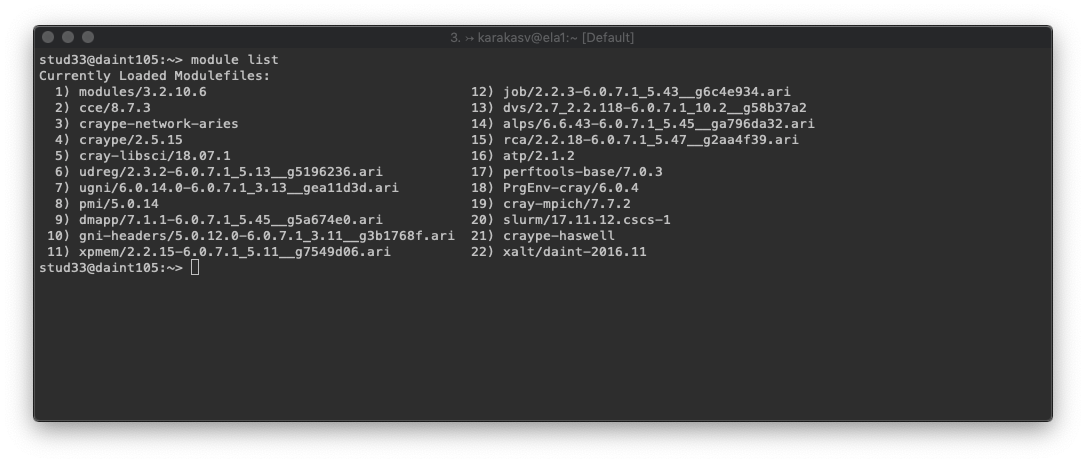
\includegraphics[width=\textwidth]{module_list.png}
  }
\end{frame}

\begin{frame}{Managing programming environments}{Switching programming environments}
  \begin{itemize}
  \item[--] Switch to the PGI programming environment
  \item[--] \shinline{module switch}
  \end{itemize}
  {
    \centering
    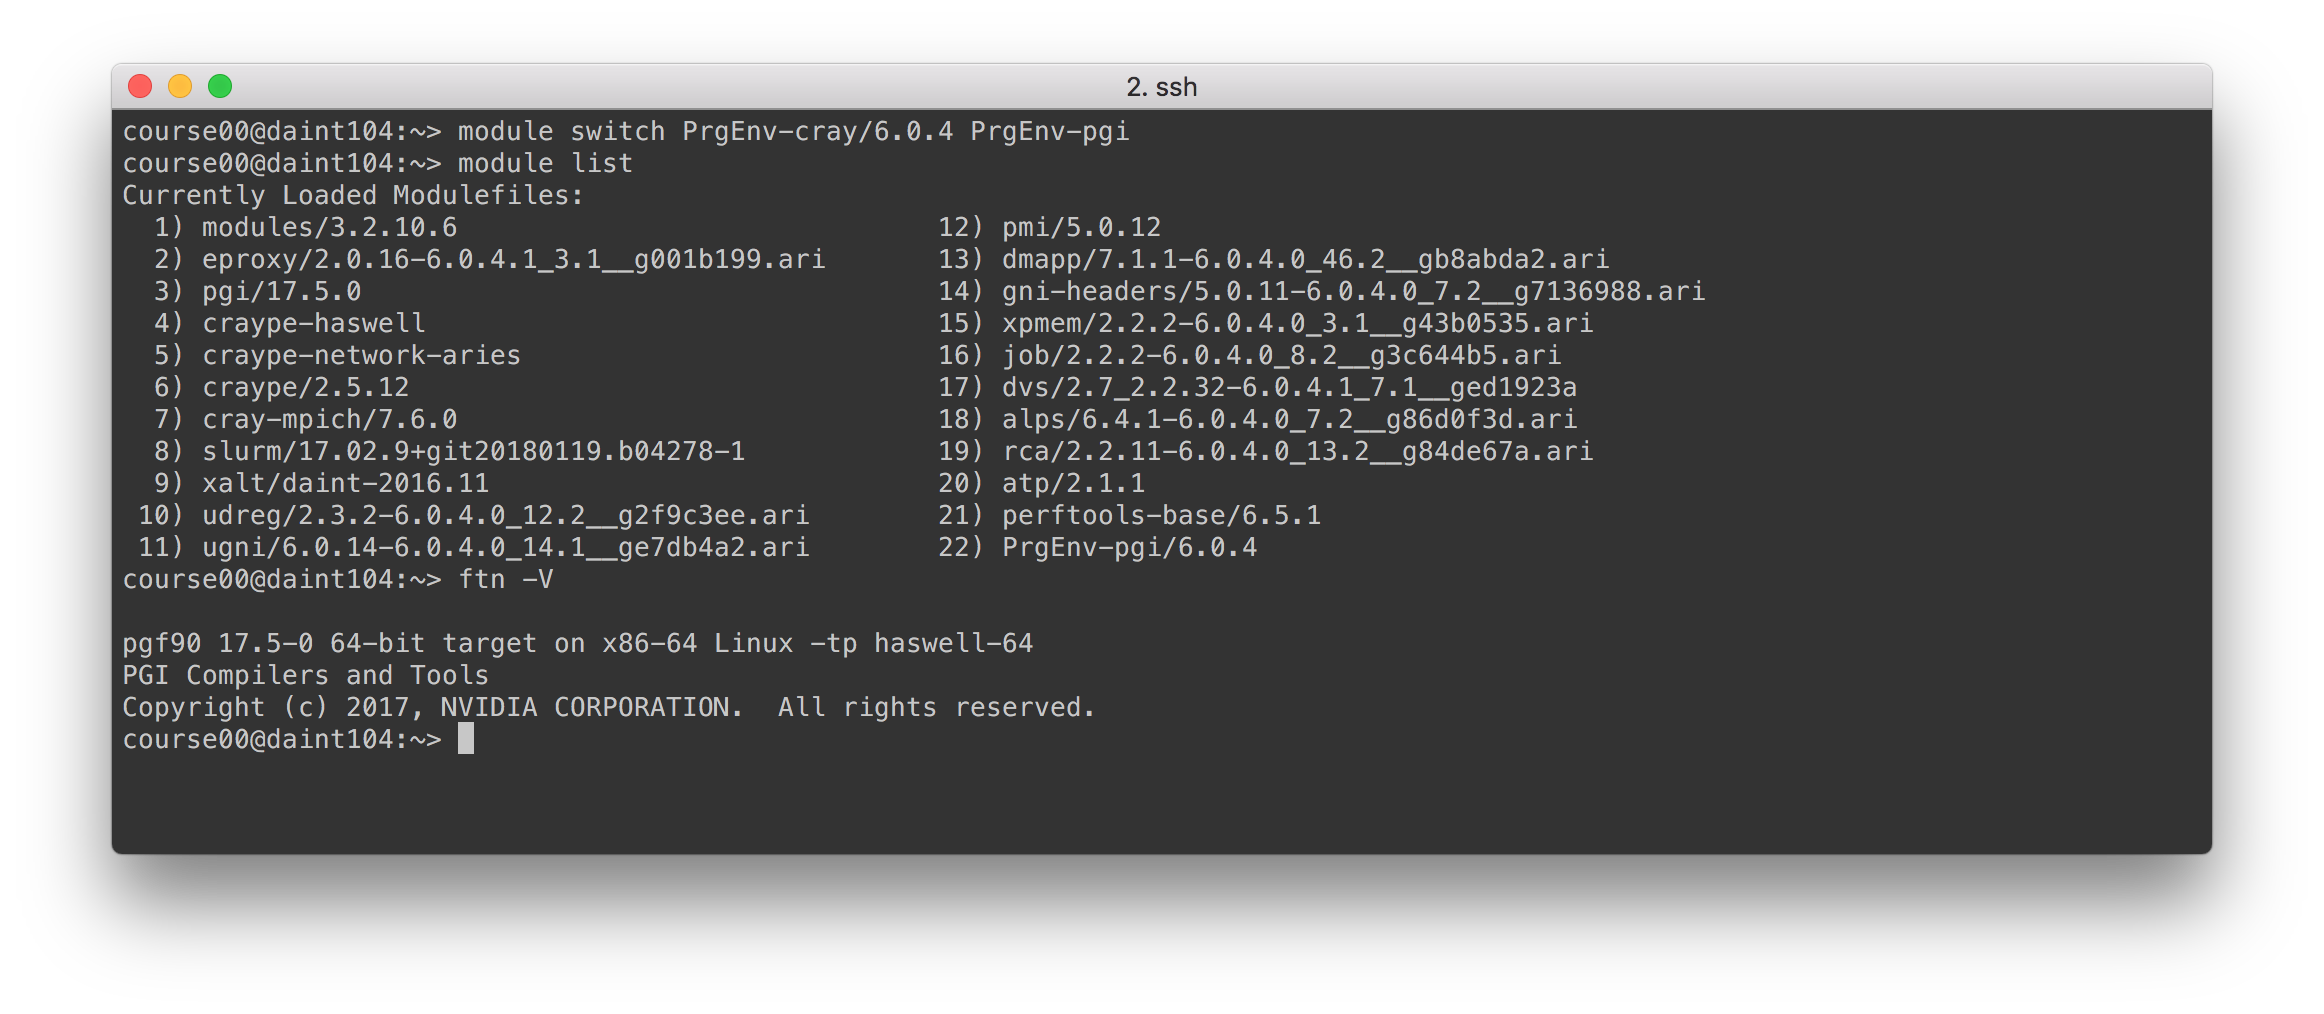
\includegraphics[width=\textwidth]{module_switch.png}
  }
\end{frame}

\begin{frame}{Managing programming environments}{Switching back to the Cray programming environment}
  {
    \centering
    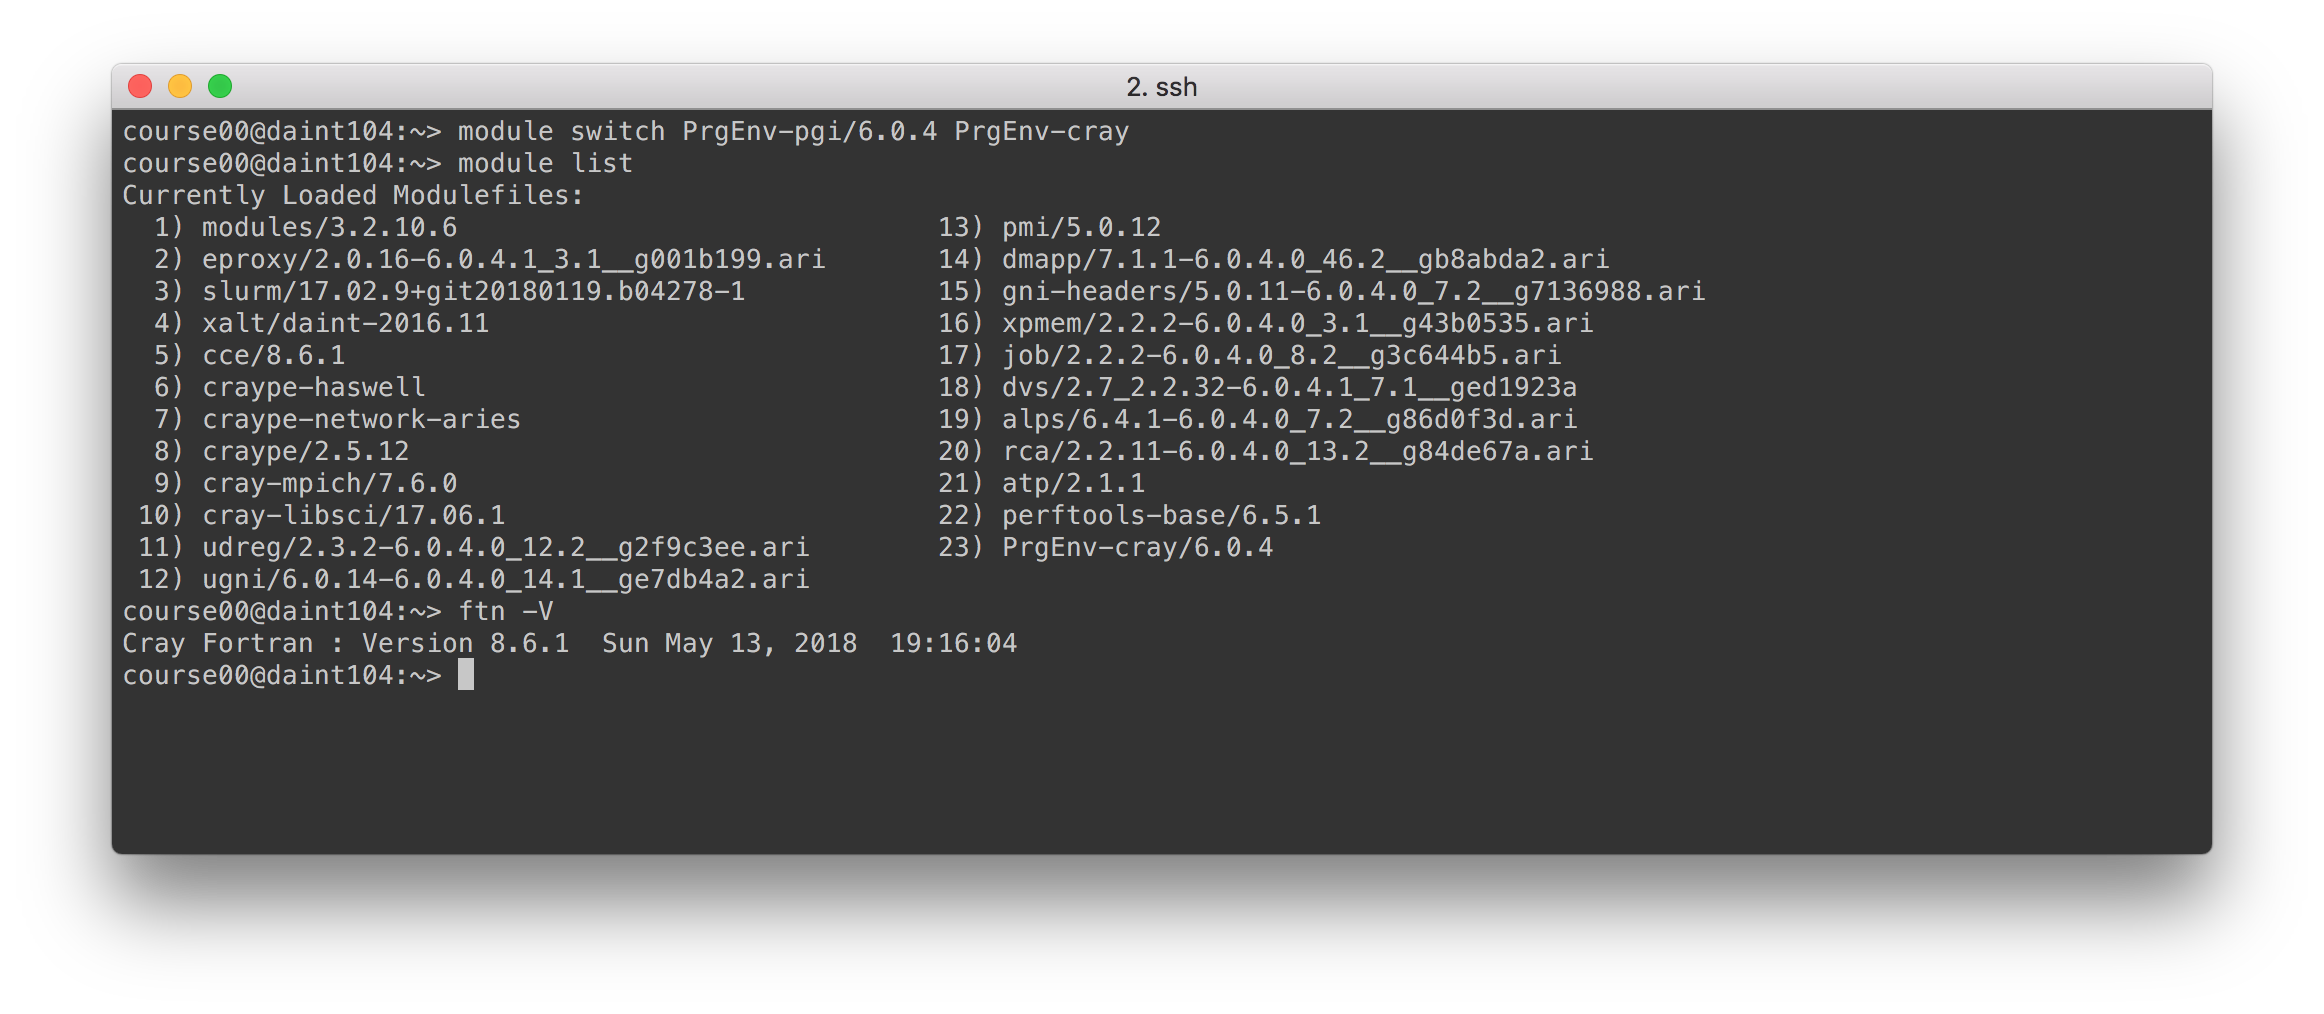
\includegraphics[width=\textwidth]{module_switch_cray.png}
  }
\end{frame}

\begin{frame}{Managing programming environments}{Loading and unloading modules}
  \begin{itemize}
  \item[--] \shinline{module load [MODULE_NAME]}
  \item[--] \shinline{module unload [MODULE_NAME]}
  \end{itemize}

  {
    \centering
    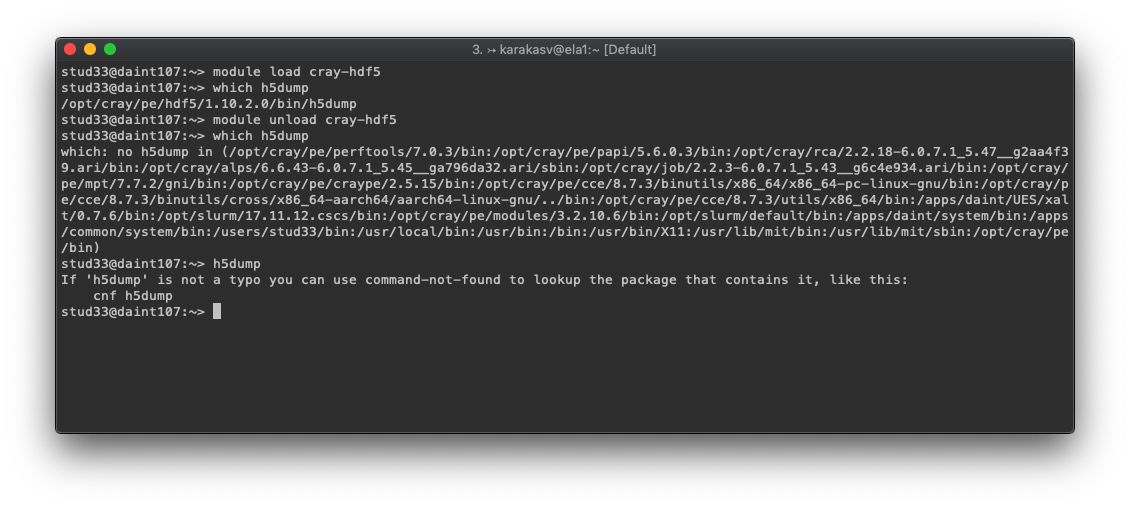
\includegraphics[width=\textwidth]{module_load_unload.png}
  }
\end{frame}


\begin{frame}{Managing programming environments}{Checking available modules}
  \begin{itemize}
  \item[--] The \texttt{daint-gpu} makes available the CSCS software stack built for the hybrid nodes of the system
  \end{itemize}
  {
    \centering
    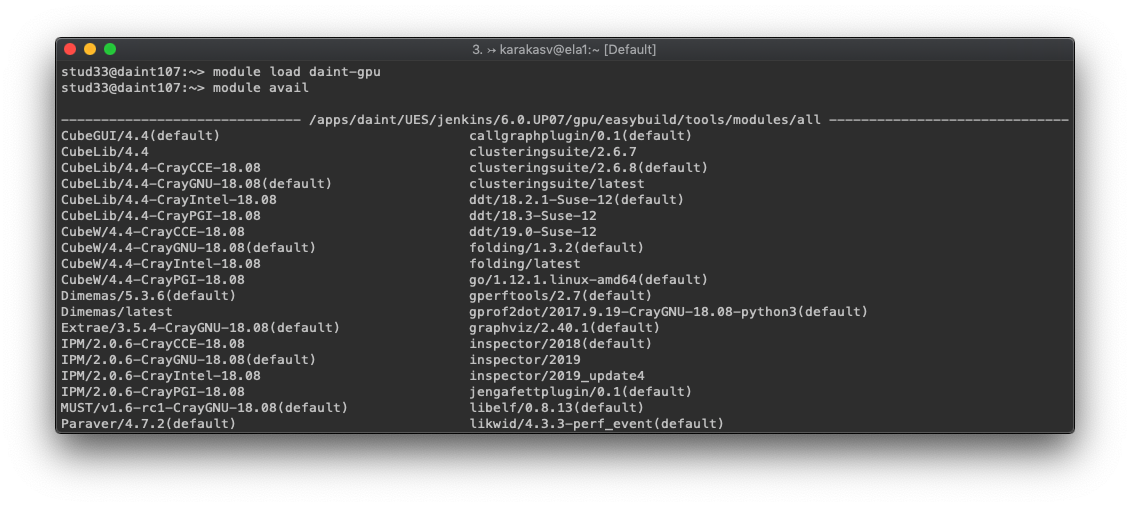
\includegraphics[width=\textwidth]{module_avail_all.png}
  }
\end{frame}

\begin{frame}{Managing programming environments}{Checking available modules}
  \begin{itemize}
  \item Check available versions of a software
  \end{itemize}
  {
    \centering
    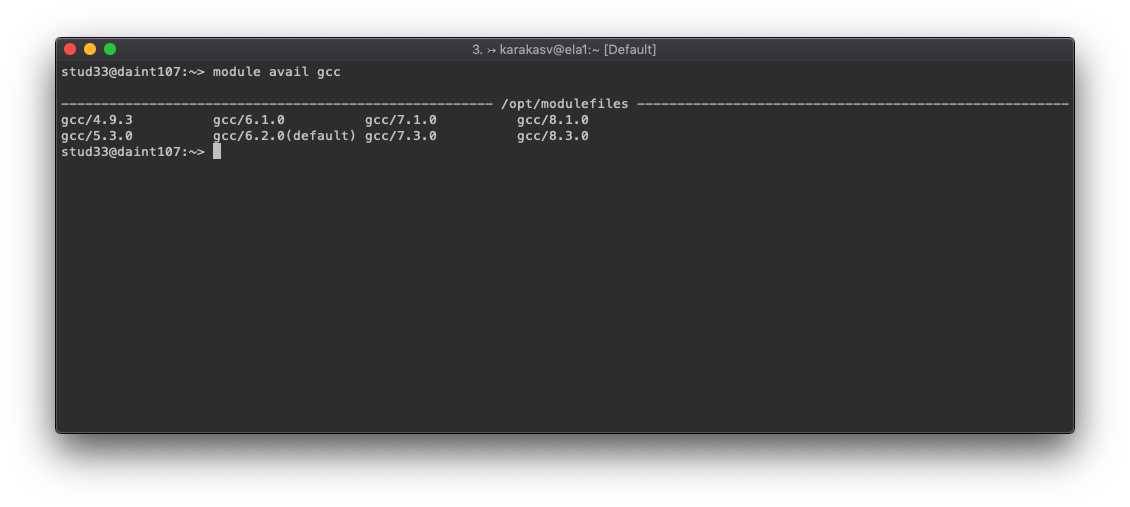
\includegraphics[width=\textwidth]{module_avail_gcc.png}
  }
\end{frame}

\begin{frame}{Managing programming environments}{Get information about a module}
  \begin{itemize}
  \item[--] Environment variables set, paths etc.
  \end{itemize}

  {
    \centering
    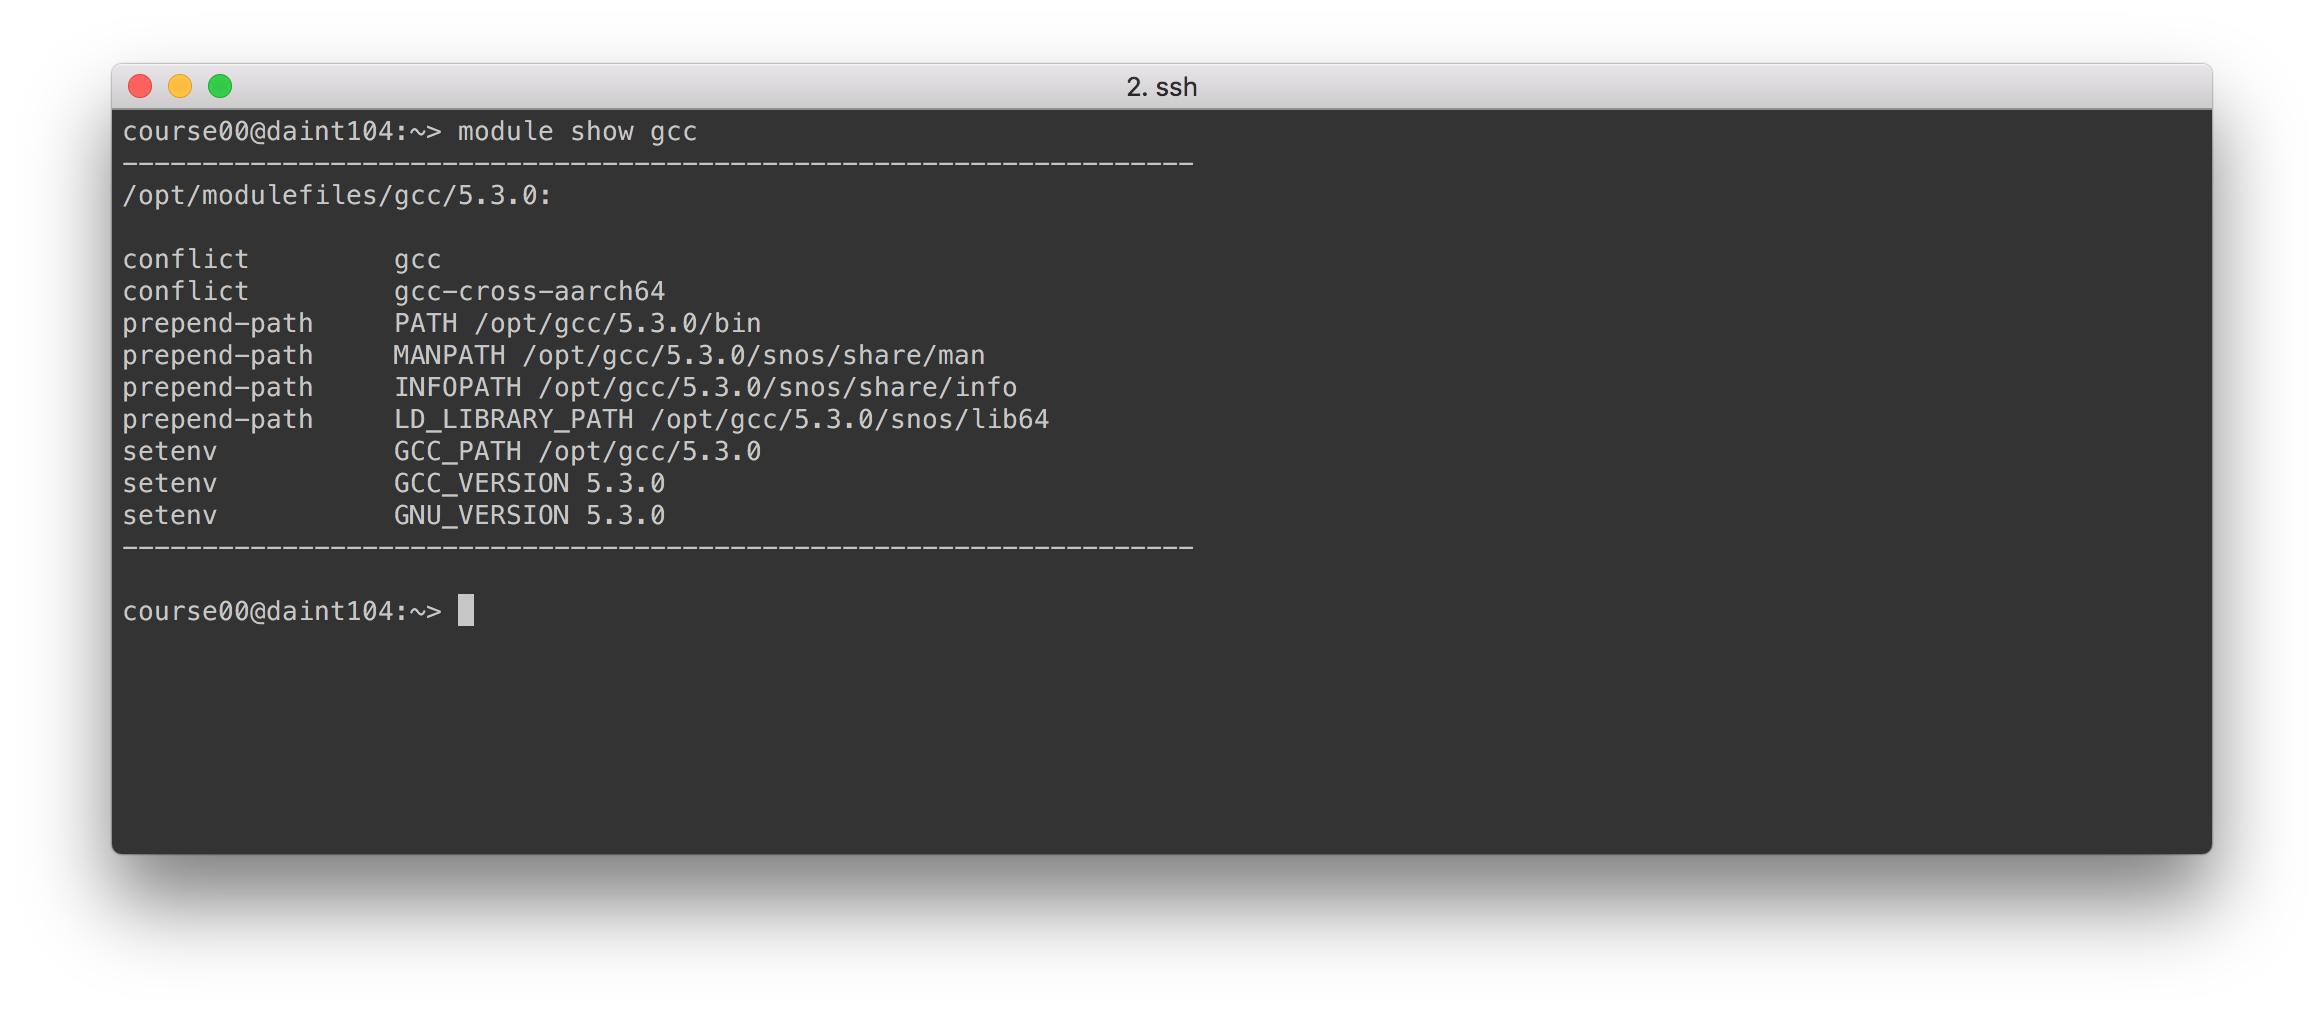
\includegraphics[width=\textwidth]{module_show_gcc.png}
  }
\end{frame}


\begin{frame}{Managing programming environments}{Get help for a module}
  {
    \centering
    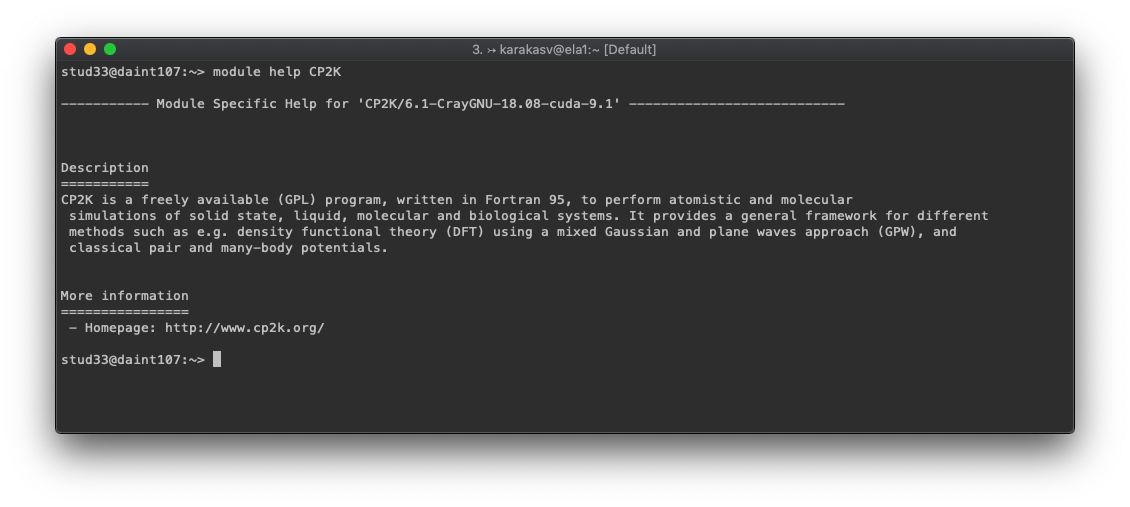
\includegraphics[width=\textwidth]{module_help_cp2k.png}
  }
\end{frame}
